\section{Analytical Insights}\label{sec:analytic}
Closed forms (F1--F8) explain the simulations, serve as fast surrogates and check the solver. Numbers refer to
RP-63 (\cref{sec:params}), new, at 25\,$^\circ$C unless stated; scenarios S1--S16 are defined in
\cref{sec:usage}.

\paragraph{F1: energy bucket (L0).}
The usable energy is $E_u(\soc_0)=Q_{\max}\int_{\soc_e}^{\soc_0}\Ocv(\zeta)\,\dd\zeta$ ($E_u(1)=17.8$\,W\,h), and
$\TTE_0=E_u/\bar P$. If $P=\sum_iP_i$ and $\phi_i$ is component $i$'s share of the energy, then
$\partial\ln\TTE_0/\partial\ln P_i=-\phi_i$, and removing $i$ multiplies $\TTE_0$ by $1/(1-\phi_i)$: the energy pie
chart \emph{is} the sensitivity chart. For the scheduled day (S12) the shares range from processor 40.0\,\%,
display 27.2\,\% and radio 14.5\,\% down to sensors 0.6\,\%. Each 10\,\% saved on the display gains about 2.8\,\% of runtime; no
sensor setting can matter.

\paragraph{F2: exact quadrature (L1).}
For constant $P$ and $T$ with the RC branch in equilibrium ($R_\Sigma=R_0+R_1$), $\dd t=-Q_{\max}\,\dd\soc/I$ and
$1/I=V/P$ give the time in hours to reach SOC $\soc$:
\begin{equation}
  t(\soc)=\frac{Q_{\max}}{P}\int_{\soc}^{\soc_0}V_{\mathrm{qs}}\,\dd\zeta,\quad
  V_{\mathrm{qs}}=\tfrac12\Big(\Ocv+\sqrt{\Ocv^2-4R_\Sigma P}\Big),\quad
  \TTE=t(\soc_c),\quad \Ocv(\soc_c)=\Vcut+\frac{P\,R_\Sigma(\soc_c)}{\Vcut}. \label{eq:F2}
\end{equation}
Since $t(\soc)$ is monotone, $\soc(t)$ follows by inversion. \Cref{eq:F2} matches the isothermal L2 model within
0.0009\,\% at 25\,$^\circ$C for 0.5--3.5\,W (0.053\,\% at $-20\,^\circ$C, where the RC branch is slow). At the thermal steady state it matches the full
L2 TTE within 0.04\,\% for every unthrottled constant load, while L0 is at most 1.9\,\% too long; F2 is the
surrogate used in \cref{sec:uq}.

\paragraph{F3: resistive correction.}
To first order in $P$,
\begin{equation}
  E_u(P)\approx E_{u0}(1-\alpha P),\qquad
  \alpha=\frac{\int_{\soc_e}^{1}R_\Sigma/\Ocv\,\dd\soc+R_\Sigma(\soc_e)/\Ocv'(\soc_e)}{\int_{\soc_e}^{1}\Ocv\,\dd\soc},\qquad
  \frac{\partial\ln\TTE}{\partial\ln P}=-1-\frac{\alpha P}{1-\alpha P}. \label{eq:F3}
\end{equation}
The two terms are the ohmic loss and the charge left behind when the sagging voltage reaches $\Vcut$ early:
$\alpha=0.004954+0.003223=0.008177$\,W$^{-1}$. The exact L1 losses are 0.41/0.89/3.15\,\% at 0.5/1.06/3.5\,W (first
order: 2.86\,\% at 3.5\,W). Because $R_0$ rises in the cold and near empty (\cref{fig:cell_maps}b), the coefficient grows $\times2.1$ at 0\,$^\circ$C, $\times2.9$ at $-10\,^\circ$C,
$\times4.2$ at $-20\,^\circ$C, $\times1.5$ at SOH 0.8 and $\times6.3$ at $-20\,^\circ$C with SOH 0.8. Even then the loss on the social feed stays below 6\,\%: the large cold losses (\cref{sec:aging}) come from the brown-out (F4).

\begin{figure}[t]
  \centering
  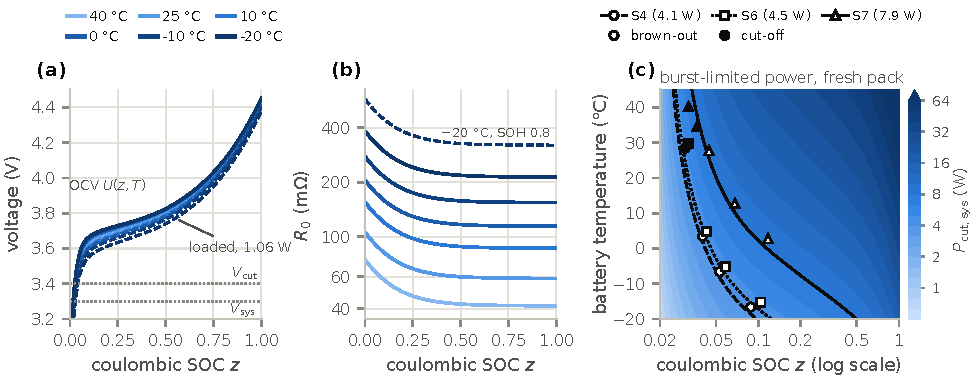
\includegraphics[width=0.95\textwidth]{figures/fig_cell_maps.pdf}
  \caption{(a) The OCV barely depends on temperature; the voltage under 1.06\,W fans out as the cell cools.
  (b) $R_0$ rises in the cold and near empty (dashed: $-20\,^\circ$C, SOH 0.8). (c) Largest sub-second peak (fresh
  pack), F4 brown-out boundaries of three loads (legend: $P+\Delta P_b$) and L2 shutdown points: every brown-out
  (open) lies on its line.}
  \label{fig:cell_maps}
\end{figure}

\paragraph{F4: brown-out, stranded charge and safe bursts.}
Setting $V_{\mathrm{pk}}=V_{\mathrm{sys}}$ in \cref{eq:burst} ($v_1\approx R_1P/\Ocv$; from here on $\Delta P_b$
includes $m_b$) gives the brown-out SOC, the stranded charge \cite{LEE20} and the safe burst:
\begin{equation}
  \Ocv(\soc^*,T)=V_{\mathrm{sys}}+v_1+\frac{R_0(\soc^*,T)(P+\Delta P_b)}{V_{\mathrm{sys}}},\qquad
  s_{\mathrm{off}}\approx\frac{\soc^*-\soc_e}{1-\soc_e},\qquad
  \Delta P_{b,\mathrm{safe}}=\frac{V_{\mathrm{sys}}(\tilde U-V_{\mathrm{sys}})}{R_0}-P. \label{eq:F4}
\end{equation}
On the social load at $-20\,^\circ$C (battery at $-16.6\,^\circ$C), $\soc^*=0.0881$ gives $s_{\mathrm{off}}=6.35$\,\%
against 6.38\,\% from the ODE. Over 5 temperatures $\times$ 3 SOH levels, F4 is within 0.17 points of L2 in all 14
brown-out cells, and every L2 brown-out lies on its F4 boundary (\cref{fig:cell_maps}c). The safe burst on
the social load at $\soc=0.5/0.2/0.1$ falls from 27.1/17.4/12.7\,W (25\,$^\circ$C, new) to 3.9/2.2/1.4\,W
($-20\,^\circ$C, SOH 0.8). At $\soc=0.5$ the largest power held for minutes, $\Vcut(\Ocv-\Vcut)/R_\Sigma$, falls
from 20.2 to 3.2\,W, and the largest sub-second peak $V_{\mathrm{sys}}(\Ocv-V_{\mathrm{sys}})/R_0$ from 28.3 to
5.3\,W. Multi-second loads end at the cut-off: the 30\,s, 4.1\,W photo burst of the cold hike lies between the
cut-off powers with $R_0$ alone (4.4\,W) and with $R_0+R_1$ (3.2\,W); as $v_1$ builds up ($\tau_1\approx2$\,min at
$-18\,^\circ$C) the voltage reaches $\Vcut$ after 24\,s, which is why the hike ends at 44\,\% displayed charge
(\cref{sec:aging}). Applied online, F4 is the burst governor of \cref{sec:recs}.

\paragraph{F5: thermal cap.}
When the skin limit binds, the thermal node settles at a fixed point
\begin{equation}
  T_s^*=\Tamb+k_{\mathrm{env}}R_{\mathrm{skin}}\big[P(T_s^*)+q_{\mathrm{batt}}\big],\quad P^*=P(T_s^*),\quad
  \TTE_{\mathrm{cap}}\approx\frac{E_u}{P^*},\quad
  \frac{\dd\TTE_{\mathrm{cap}}}{\dd\Tamb}\approx\frac{E_u}{P^{*2}}\,\frac{G}{1+k_{\mathrm{env}}R_{\mathrm{skin}}G}>0, \label{eq:F5}
\end{equation}
with $G=(P_{\mathrm{SoC,dem}}-P_{\mathrm{fl}})\,\sigma(1-\sigma)/w_{\mathrm{thr}}$ from \cref{eq:throttle}. As
$w_{\mathrm{thr}}\to0$ the slope tends to the sharp-cap value $E_u/(k_{\mathrm{env}}R_{\mathrm{skin}}P^{*2})$, with
$P^*\approx(T_{\lim}-\Delta T_{\mathrm{thr}}-\Tamb)/(k_{\mathrm{env}}R_{\mathrm{skin}})$.
A \emph{hotter} room lengthens gaming time: the OS throttles harder, trading frame rate for
runtime. For the 3.91\,W game ($q_{\mathrm{batt}}$ neglected), $P^*=3.90/3.12/1.73$\,W at 15/25/35\,$^\circ$C,
with performance ratio $\rho_{\mathrm{perf}}=0.999/0.864/0.531$ and $E_u/P^*=4.56/5.71/10.3$\,h; L2 gives
4.40\,h (not throttled, ending in a brown-out), 5.68 and 10.29\,h. The slope is 0.25\,h/K at 25\,$^\circ$C and
0.74\,h/K at 35\,$^\circ$C (sharp-cap bound 0.33 and 1.08\,h/K; L2 secant 0.46\,h/K). The close match at 25\,$^\circ$C is partly a cancellation: neglecting battery
heat overstates $P^*$ (L2 delivers 3.06\,W) while L0 ignores resistive loss; F2 at $P^*$ gives 5.58\,h ($-1.8$\,\%).

\paragraph{Random usage (F6--F8).}
Let $X(t)$ be the usage CTMC (generator $\Lambda$, stationary law $\pi$, state powers $P_x$ at their thermal fixed
points), so that $\dd E/\dd t=-P_{X(t)}$ is a PDMP with $\bar P=\pi^{\top}P$. Let $h=Z(P-\bar P\mathbf 1)$, with
deviation matrix $Z=(\mathbf 1\pi^{\top}-\Lambda)^{-1}-\mathbf 1\pi^{\top}$, be the extra energy a phone now in
state $x$ will use. Dynkin's formula at the stopping time TTE (F6) and the central limit theorem (F7) give
\begin{equation}
  \mathbb E[\TTE\mid x_0]=\frac{E_u-h_{x_0}+\mathbb E[h(X_{\TTE})]}{\bar P},\qquad
  \mathrm{Var}(\TTE)\approx\frac{\sigma^2E_u}{\bar P^3},\qquad \sigma^2=2\sum_x\pi_x(P_x-\bar P)h_x, \label{eq:F6}
\end{equation}
where the approximation $\mathbb E[h(X_{\TTE})]\approx\sum_x\pi_xP_xh_x/\bar P$ reflects an inspection paradox:
batteries tend to die during high-power sessions ($h>0$). For the typical profile of \cref{sec:usage}
($\bar P=0.440$\,W, 6.5\,h screen-on per day) the fluid mean $E_u/\bar P$ is 40.43\,h and F6 gives 41.25\,h,
against $41.30\pm0.05$\,h (mean $\pm$ standard error) from 20\,000 Monte Carlo paths of L0. For the heavy profile
(0.822\,W, 11.5\,h) the values are 21.63, 22.50 and $22.45\pm0.04$\,h. On 2000 shared paths L2 is 3.6\,\%
(typical) and 4.4\,\% (heavy) shorter than L0. F7 gives SDs of 7.21\,h (CV 0.175) and 5.18\,h (CV 0.230), 2.2 and
1.4\,\% above Monte Carlo. The simulated TTE is nearly symmetric, so a normal law fits better than the
inverse-Gaussian diffusion limit (quantile errors $\le0.35$\,h vs.\ up to 1.7\,h).

F8 attributes the spread. With sessions starting from idle at rate $\lambda_{\mathrm{on}}$ (activity $j$:
probability $p_j$, mean duration $d_j$; mean cycle length $\mathbb E[L]$),
$\sigma^2=2\sum_jp_jd_j^2(P_j-\bar P)^2/\mathbb E[L]$ and
$\partial\ln(E_u/\bar P)/\partial\ln d_j=-\pi_j(P_j-\bar P)/\bar P$. Long, high-power sessions dominate: gaming
uses 28\,\% of the typical energy but causes 81\,\% of the variance (heavy: 94\,\%). The usage elasticities of the
mean are $-0.53$ (session rate), $-0.26$ (game length), $-0.17$ (social length) and $+0.065$ (audio length). A
longer screen-off music session thus \emph{extends} battery life: its 0.22\,W is below $\bar P$ and it postpones
the next session. Longer games shorten the mean and widen the spread (SD elasticity $+0.35$).

\begin{keybox}[Key finding]
At 25\,$^\circ$C drain is an energy problem. Beyond energy, only the cold or aged voltage limits (F4) and the
thermal cap that makes games last \emph{longer} in hot rooms (F5) matter.
\end{keybox}
